\chapter{DuckieTown}

\section{Umgebung und Simulator}


Der \href{https://github.com/duckietown/gym-duckietown}{DuckieTown-Simulator} ist ein in \href{https://www.python.org/}{\texttt{Python}} und \href{https://www.opengl.org/}{\texttt{OpenGL}} beziehungsweise \href{http://pyglet.org/}{\texttt{Pyglet}} geschriebener Simulator für das \glqq DuckieTown-Universum\grqq. Er basiert auf dem OpenAi Toolkit ``Gym'' \cite{gym} und bietet die Möglichkeit DuckieBots (Agenten) in einer beliebigen DuckieTown-Umgebung zu platzieren und die Agenten darin zu navigieren. \cite{gym_duckietown} \\

Der Simulator ist schnell, quelloffen und ausgesprochen anpassungsfähig. Er wurde zunächst für die einfache Linienverfolgung konzipiert und wurde dann im Laufe der Zeit zu einem voll funktionsfähigen Simulator für autonom fahrende Fahrzeuge, insbesondere im Bezug zur künstlichen Intelligenz. \cite{gym_duckietown}

In einer DuckieTown-Umgebung wird die Umwelt für einen DuckieBot definiert. Ein DuckieBot kann diese Umgebung dann observieren und sich in dieser bewegen. Eine DuckieTown-Umgebung wird dabei aus verschiedenen Kacheln und Objekten aufgebaut. Eine beispielhafte DuckieTown-Umgebung ist in Abbildung \ref{duckietown-env} dargestellt.

\begin{figure}[H]
	\centering
	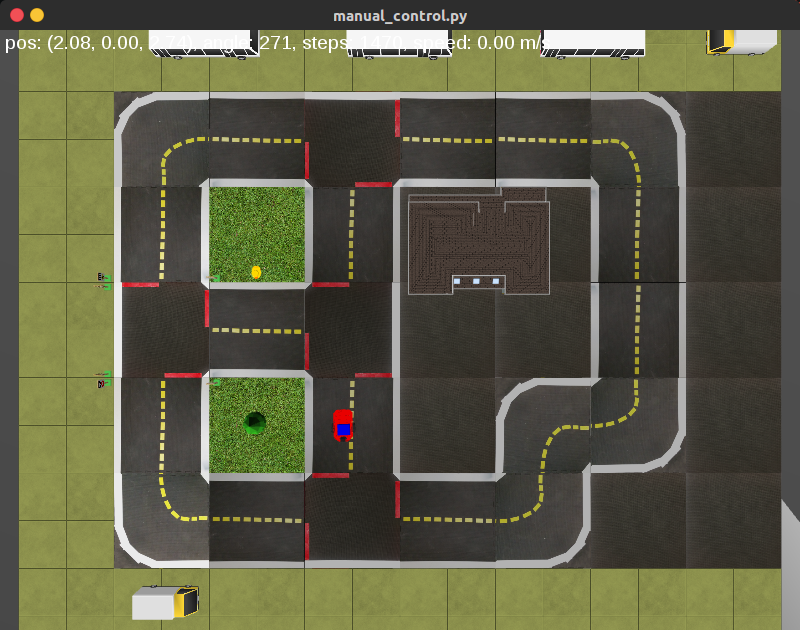
\includegraphics[width=0.6\textwidth]{kapitel2/images/duckietown-umgebung.png}
	\caption{Darstellung einer beispielhaften DuckieTown-Umgebung}
	\label{duckietown-env}
	\vspace{0.2cm}
	\quelle\url{https://user-images.githubusercontent.com/10503729/45590954-c88c7c00-b912-11e8-9209-f72924684e21.gif}
\end{figure}

Bei den Kacheln wird zwischen befahrbaren und nicht befahrbaren Kacheln unterschieden, wobei folgende Kacheln standardmäßig zur Verfügung stehen:

\begin{itemize}
	\item 
		\begin{tabular}[t]{lll}
			Leere Kachel & (nicht befahrbar) & \hspace{2.45cm} 
			$ \begin{array}{l}
				\setlength{\fboxsep}{0pt}
				\fbox{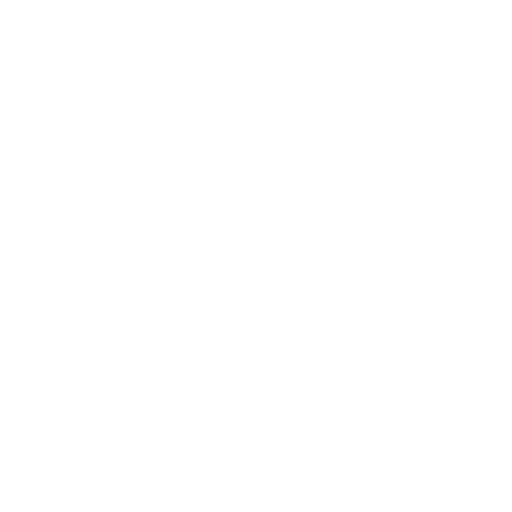
\includegraphics[scale=0.135]{kapitel2/images/empty.png}}
			\end{array} $
		\end{tabular} 
	
	\item 
		\begin{tabular}[t]{lll}
			Gerader Streckenabschnitt & (befahrbar) & \hspace{1.15cm}
			$ \begin{array}{l}
				\setlength{\fboxsep}{0pt}
				\fbox{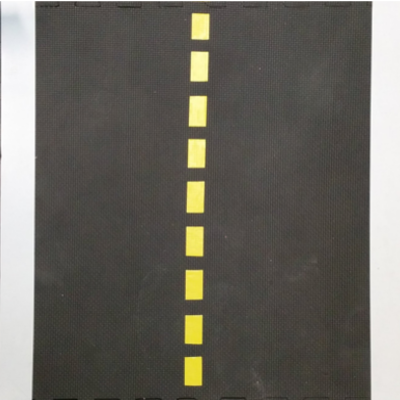
\includegraphics[scale=0.17]{kapitel2/images/straight.png}}
		  	\end{array} $
		\end{tabular}
	
	
	\item 
		\begin{tabular}[t]{lll}
			Linkskurve & (befahrbar) & \hspace{3.75cm}
			$ \begin{array}{l}
				\setlength{\fboxsep}{0pt}
				\fbox{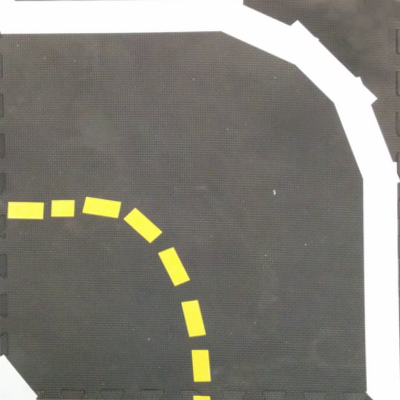
\includegraphics[scale=0.17]{kapitel2/images/left.png}}
			\end{array} $
		\end{tabular}
	
	\item 
		\begin{tabular}[t]{lll}
			Rechtskurve & (befahrbar) & \hspace{3.55cm}
			$ \begin{array}{l}
				\setlength{\fboxsep}{0pt}
				\fbox{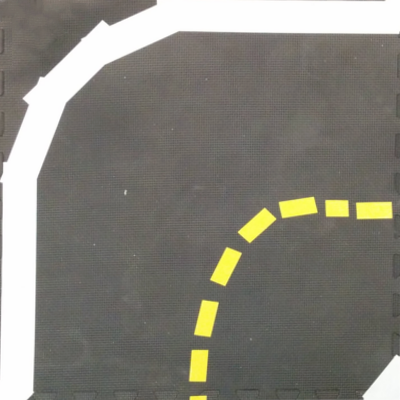
\includegraphics[scale=0.17]{kapitel2/images/right.png}}
			\end{array} $
		\end{tabular}
	
	\item 
		\begin{tabular}[t]{lll}
			3-Wege Kreuzung & (befahrbar) & \hspace{2.6cm}
			$ \begin{array}{l}
				\setlength{\fboxsep}{0pt}
				\fbox{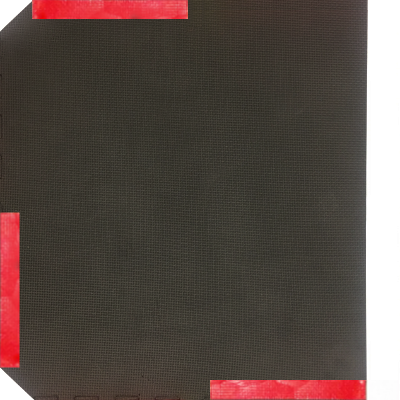
\includegraphics[scale=0.17]{kapitel2/images/3way.png}}
			\end{array} $
		\end{tabular}
	
	\item 
		\begin{tabular}[t]{lll}
			4-Wege Kreuzung & (befahrbar) & \hspace{2.6cm}
			$ \begin{array}{l}
				\setlength{\fboxsep}{0pt}
				\fbox{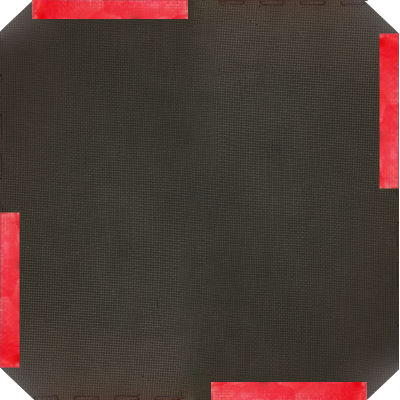
\includegraphics[scale=0.17]{kapitel2/images/4way.png}}
			\end{array} $
		\end{tabular}
	\item 
		\begin{tabular}[t]{lll}
			Asphaltkachel & (nicht befahrbar) & \hspace{2.25cm}
			$ \begin{array}{l}
				\setlength{\fboxsep}{0pt}
				\fbox{
\includegraphics[scale=0.17]{kapitel2/images/asphalt.png}}
			\end{array} $
		\end{tabular}
	
	\item 
		\begin{tabular}[t]{lll}
			Graskachel & (nicht befahrbar) & \hspace{2.75cm}
			$ \begin{array}{l}
				\setlength{\fboxsep}{0pt}
				\fbox{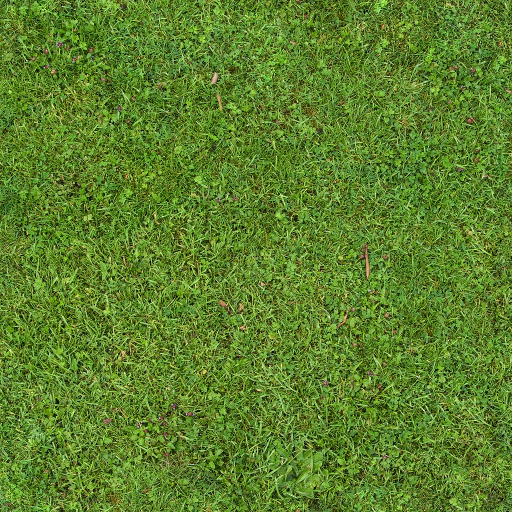
\includegraphics[scale=0.132]{kapitel2/images/grass.png}}
			\end{array} $ \\
		\end{tabular}
	
	\item 
		\begin{tabular}[t]{lll}
			Bodenkachel & (nicht befahrbar) & \hspace{2.45cm}
			$ \begin{array}{l}
				\setlength{\fboxsep}{0pt}
				\fbox{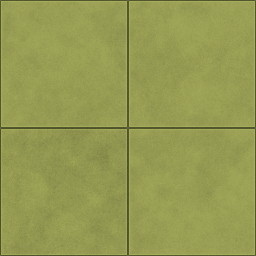
\includegraphics[scale=0.26]{kapitel2/images/floor.png}}
			\end{array} $
		\end{tabular}
\end{itemize}

Objekte sind ebenfalls nicht befahrbar und befinden sich in der Regel außerhalb des Streckenverlaufes. Standardmäßig werden eine Vielzahl von Objekten zur Verfügung gestellt, wie zum Beispiel: Häuser, Bäume, Busse und Verkehrsschilder.

Eine DuckieTown-Umgebung wird hierbei in einer \texttt{.yaml}-Datei definiert (siehe Codebeispiel \ref{duckietown-env-definition}), die dann vom Simulator geladen und dargestellt wird .

\hspace{1cm}
\begin{minipage}{.73\linewidth}
	\begin{lstlisting}[caption={Beispieldefinition einer DuckieTown-Umgebung}\label{duckietown-env-definition}, language=python]
		# 3x3 tiles with left turns at the corners
		# going in a counter-clockwise loop
	
		tiles:
		- [curve_left/W , straight/W, curve_left/N]
		- [straight/S   , asphalt   , straight/N]
		- [curve_left/S , straight/E, curve_left/E]
	
		tile_size: 1
	\end{lstlisting}
\end{minipage}

\section{DuckieBot}
\label{duckiebot}

Ein \href{https://get.duckietown.com/products/duckiebot-db18}{DuckieBot} ist ein kleiner mobiler Roboter, ausgestattet mit einem einem \href{https://www.raspberrypi.org/}{Raspberry Pi 3}, einem Differenzialantrieb und einer Raspberry Pi Kamera.
In der physikalischen Spezifikation besitzt der Roboter zur Kommunikation mit anderen Bots optional noch ein \acs{led}-Panel und \acs{wlan}-Adapter. Die Abbildung \ref{fig:duckiebot} zeigt die Darstellung eines physikalischen DuckieBots. Im Gym-DuckieTown Simulator existiert standardmäßig pro Umgebung nur ein Roboter.

\begin{figure}[H]
	\centering
	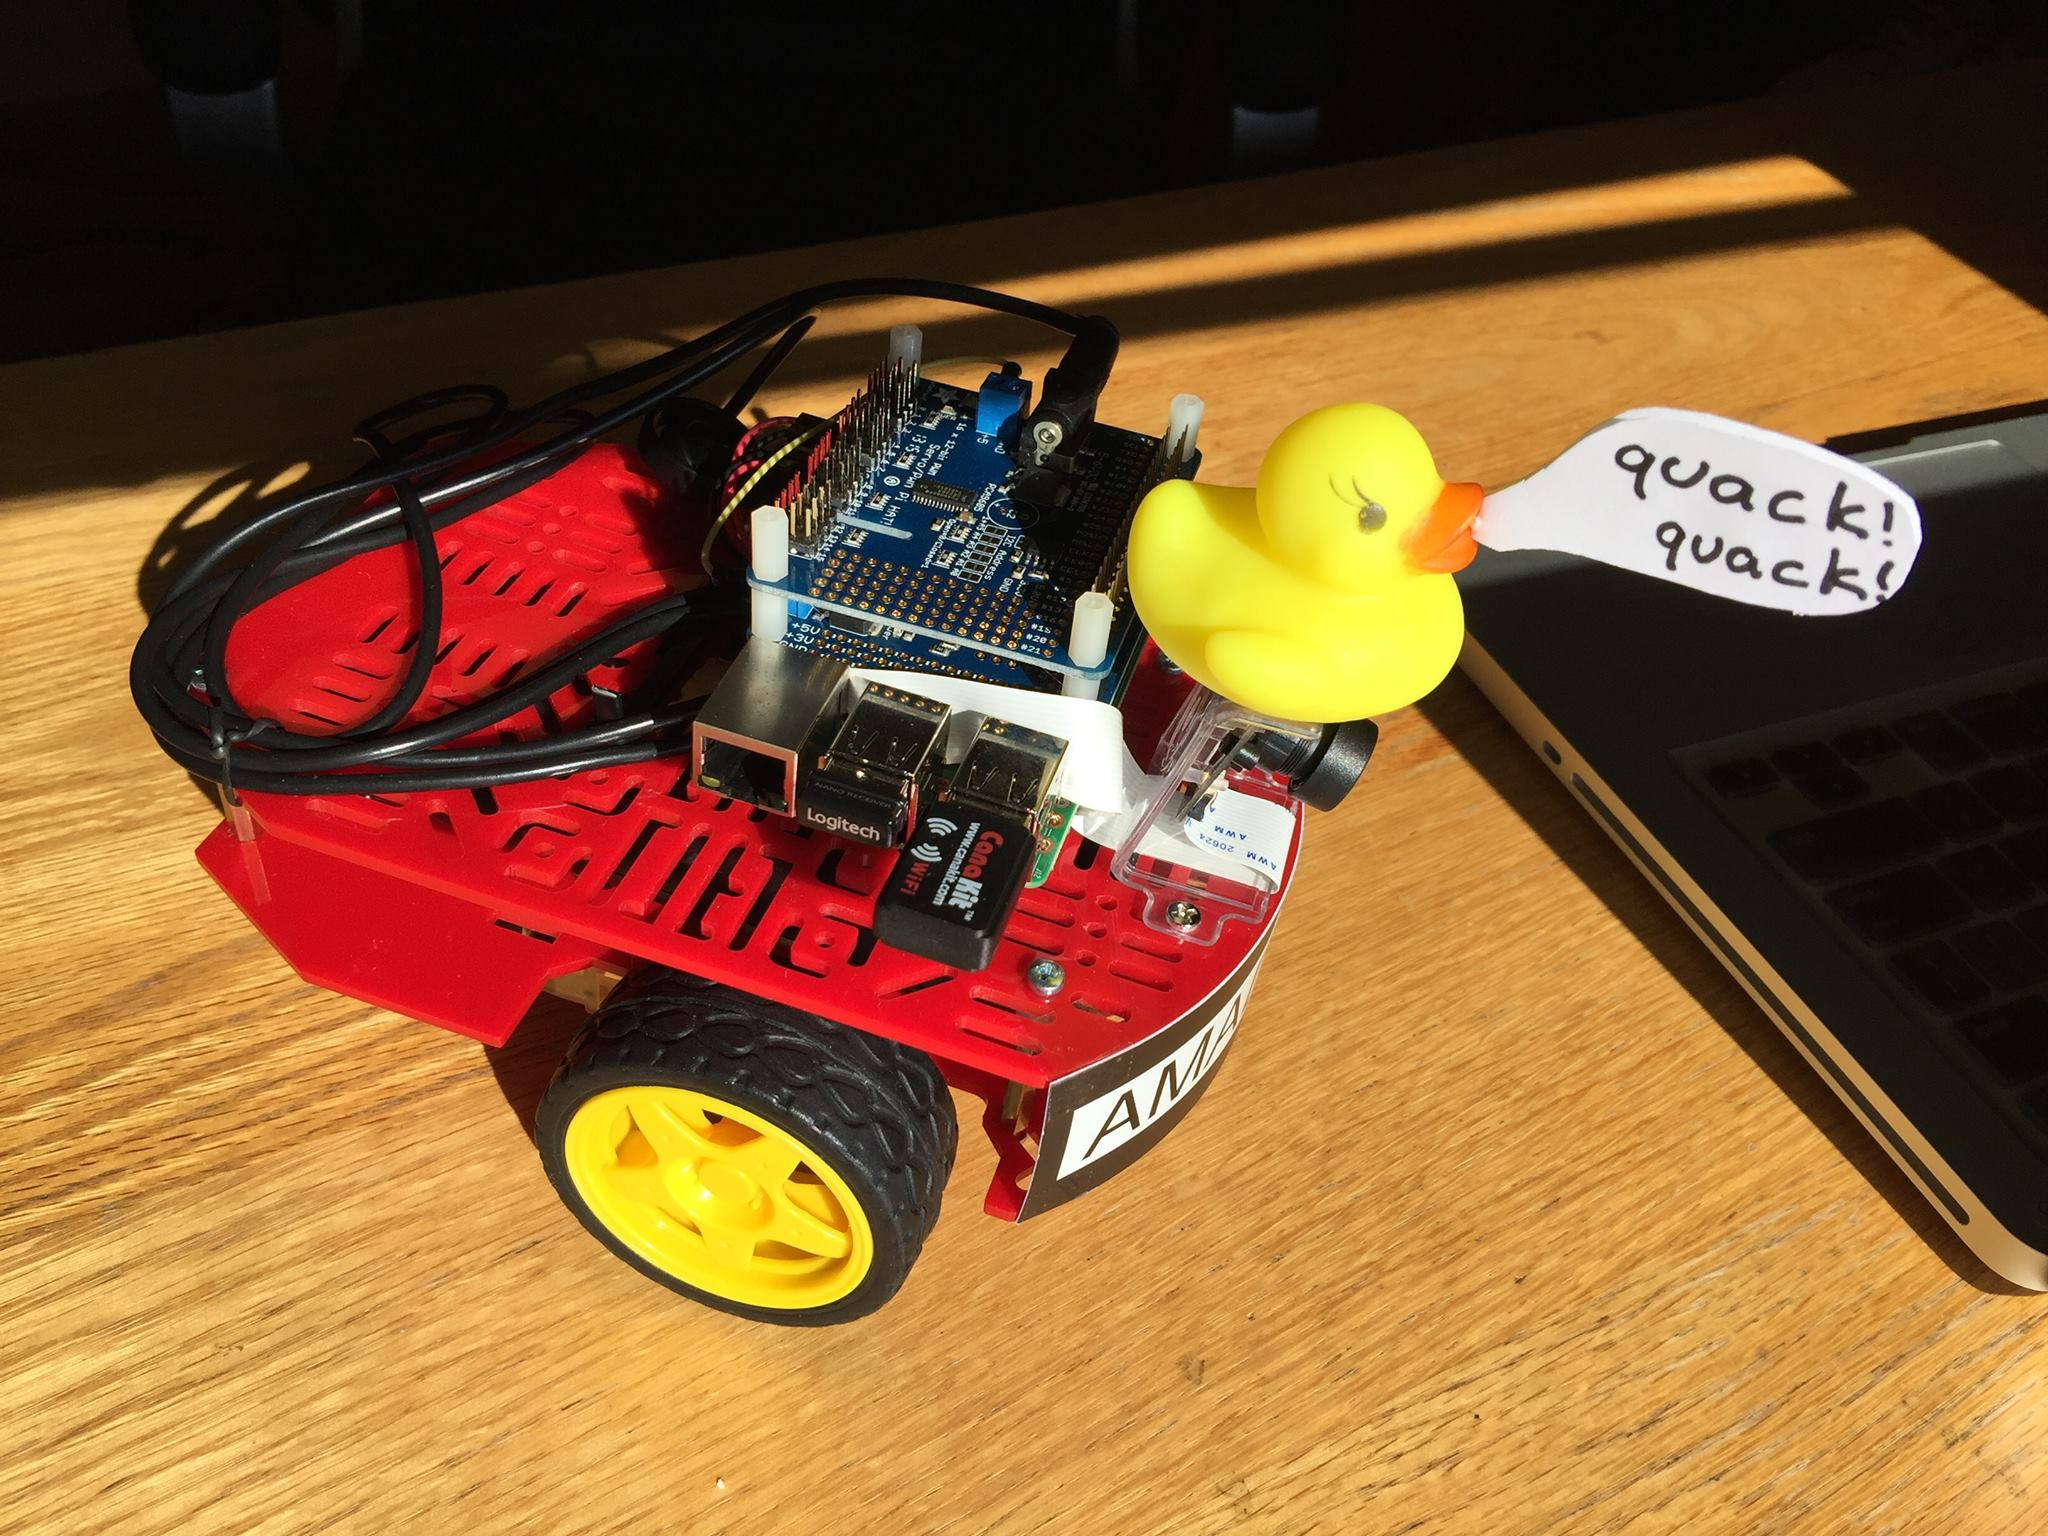
\includegraphics[width=0.5\textwidth]{kapitel2/images/duckiebot.jpg}
	\caption{Darstellung eines DuckieBots}
	\label{fig:duckiebot}
	\vspace{0.2cm}
	\quelle\url{https://cdn-blog.adafruit.com/uploads/2016/05/mercedes.jpg}
\end{figure}


\section{Bedienung}

Die Bedienung des Simulators erfolgt in einer einfachen Kontrollschleife. Zunächst wird eine \texttt{DuckieTownEnv}-Umgebung definiert und instanziiert. Anschließend wird in einer Schleife über die \texttt{step(action)} Methode der Agent gesteuert. Da die  \texttt{DuckieTownEnv}-Umgebung einen Differenzialantrieb simuliert, ist \texttt{action} dabei ein Tupel aus Geschwindigkeit und Winkelgeschwindigkeit. Die Basisklasse \texttt{Simulator} dagegen nimmt zwei Werte als Dutycycle im Wertebereich -1 bis 1 für die beiden Antriebe entgegen.

\begin{minipage}{\linewidth}
	\begin{lstlisting}[caption={Bedienung einer DuckieTown-Umgebung},
	,label={pd-drive-example}, language=Python]
	env = DuckietownEnv()
	obs = env.reset()
	env.render()
	
	while True:
		
		lane_pose = get_lane_pos(env)
		steering = k_p * lane_pose.dist + k_d * lane_pose.angle_rad
		obs,reward,done,info = env.step(np.array([speed, steering]))
		env.render()
		
		if done:
			env.reset()
	
	\end{lstlisting}
\end{minipage}

Über die Methode \texttt{reset()} wird der Agent in einer zufälligen aber validen Pose platziert, also an einem befahrbaren und nicht durch andere Objekte besetzten Ort. Mit \texttt{render()} wird ein \acs{gl}-Fenster geöffnet und ein Bild aus der Perspektive des Agenten angezeigt.\\

Die Methode \texttt{get\_lane\_pos(env)}, auch gerne ``Cheat-Modul'' genannt, liefert Poseninformationen des Agenten relativ zur Fahrbahn. Diese bestehen aus dem Abstand zur ``Ideallinie'', dem Abstand zur rechten Fahrbahnmarkierung, dem Skalarprodukt aus Richtungsvektor des Agenten und Tangente der Ideallinie am nächstgelegenen Punkt, sowie Winkeldifferenz (Arcuscosinus des Skalarprodukts).\\

Die Steuerung des Agenten erfolgt in diesem Beispiel über einen einfachen \acs{pd}-Regler, wobei der Abstand zur Ideallinie \texttt{lane\_pose.dist} als Fehler zum Sollwert interpretiert wird und die Differenz der Orientierungen von Agent und Fahrspur \texttt{lane\_pose.angle\_rad} als Ableitung des Fehlers.\\

Entgegengenommen wird der Steuerbefehl von der \texttt{step()} Methode des Simulators. Diese integriert den Befehl über eine definierte Zeitspanne \texttt{delta\_time}, standardmäßig festgelegt als der Kehrwert der Bildrate des Simulators von 30 Bildern pro Sekunde. Zurück liefert die Methode eine \acs{rgb}-Bildaufnahme aus Perspektive des Agenten (\texttt{obs}), einen Belohnungswert \texttt{reward} für das Halten der Spur und Vermeiden von Kollisionen, ein Flag \texttt{done}, welches anzeigt ob der Agent ``verunglückt'' ist und neu platziert werden muss, und das Wörterbuch \texttt{info} mit Zustandsinformationen des Agenten.\\

Das Ziel unseres Teams ist aus dem \acs{rgb}-Bild \texttt{obs} den Wert \texttt{steering} zu inferieren.